% Copyright 2019 Clara Eleonore Pavillet

% Author: Clara Eleonore Pavillet
% Description: This is an unofficial Oxford University Beamer Template I made from scratch. Feel free to use it, modify it, share it.
% Version: 1.0

\documentclass{beamer}
\usepackage{pdfpages}
% Load Packages
\usepackage[utf8]{inputenc}
\usepackage{xcolor}
\usepackage{tikz}
\usetikzlibrary{positioning,calc}
\usepackage{graphicx}
\usepackage{hyperref}
\usepackage{amsmath}
\usepackage{listings}
\usepackage{fontawesome}
\usepackage[T2A]{fontenc}
\usepackage[utf8]{inputenc}
\usepackage[russian]{babel}

% Define Commands
\newcommand*{\ClipSep}{0.06cm} %To adjust footer logo
\newcommand{\E}{\mathrm{e}\,} %\def\I{e} % used to defined e for exp(x), see later what it should be
\newcommand{\ud}{\mathrm{d}}
\lstset{numbers=left, numberstyle=\tiny, stepnumber=1,firstnumber=1,breaklines=true,
    numbersep=5pt,language=Python,
    stringstyle=\ttfamily,
    basicstyle=\footnotesize, 
    showstringspaces=false
}

\usetheme{oxonian}
\usepackage{wrapfig}
\usepackage{listings}

\title{Решаване на задачи с OpenMP. Пример: \textit{класическата} задача за много тела.}
\subtitle{\textit{Курс „Паралелно програмиране“}}
\titlegraphic{{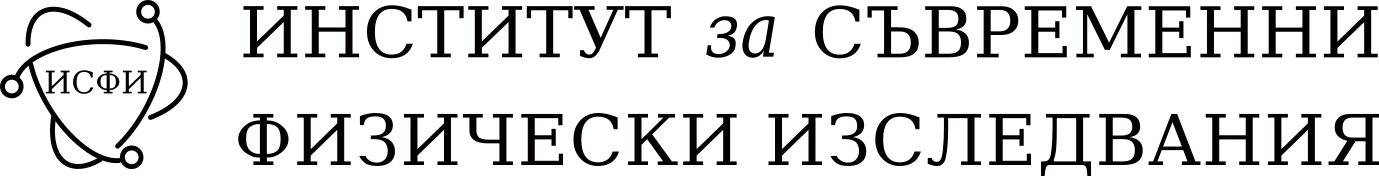
\includegraphics[width=5.3cm]{iaps.png}}} 

\author{\newline \newline Стоян Мишев}

\vspace{1cm}

\date{} %\today

\begin{document}
\lstset{language=Python}
{\setbeamertemplate{footline}{} 
\frame{\titlepage}}


\section*{План}\begin{frame}{План}\tableofcontents\end{frame}

%%%%%%%%%%%%%%%%%%%%%%%%%%%%%%%%%%%%%%%%%%%%%%%%%%%
\begin{frame}
  \frametitle{Определяне на задачата.}
  При дадени повече от две материални точки $i$ с маси $m_i$ и начални
  координати $r_i$ и скорости $v_i$, взаимодействащи със сила $f_{ij}$
  между тях, да се определят координатите и скоростите им във всеки
  следващ момент.
\end{frame}

\begin{frame}
  \frametitle{Определяне на задачата.}
  Гравитационна сила:


  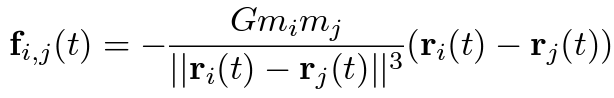
\includegraphics[width=0.65\textwidth]{force1} \pause

  Общата сила, действаща на дадена точка в момент $t$ 

  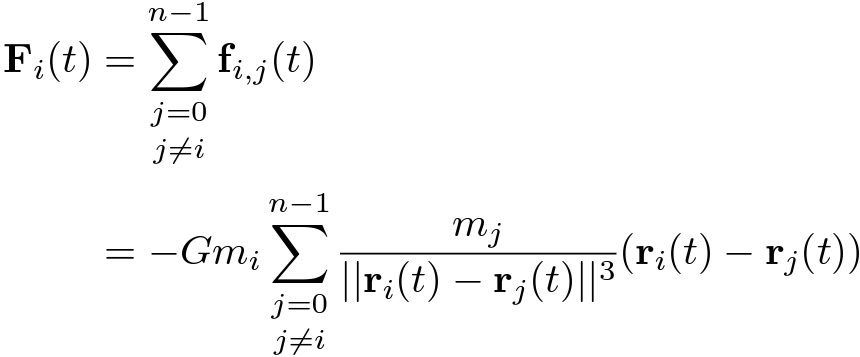
\includegraphics[width=0.8\textwidth]{force2}
\end{frame}

\begin{frame}
  Движението $r(t)$ се определя от 
  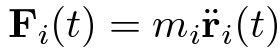
\includegraphics[width=0.22\textwidth]{force3} (Нютон). \pause

  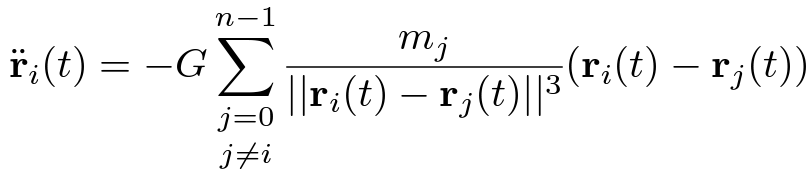
\includegraphics[width=0.62\textwidth]{accel}

  За улеснение разглеждаме движение в $R^2$.

  ``Дискретизираме'' времето $t=N\Delta t$
\end{frame}


\begin{frame}
  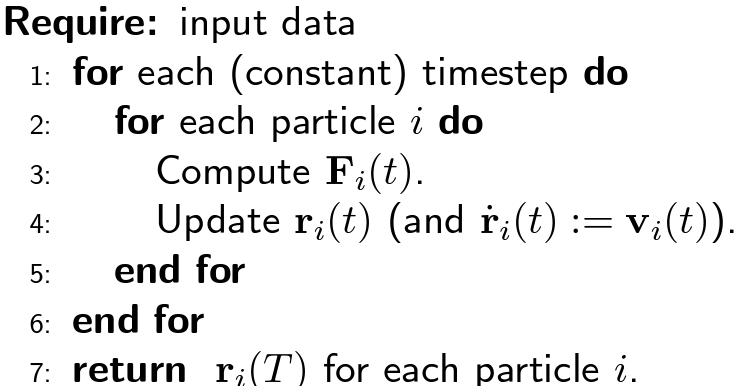
\includegraphics[width=0.6\textwidth]{pseudo-code}\pause
  
  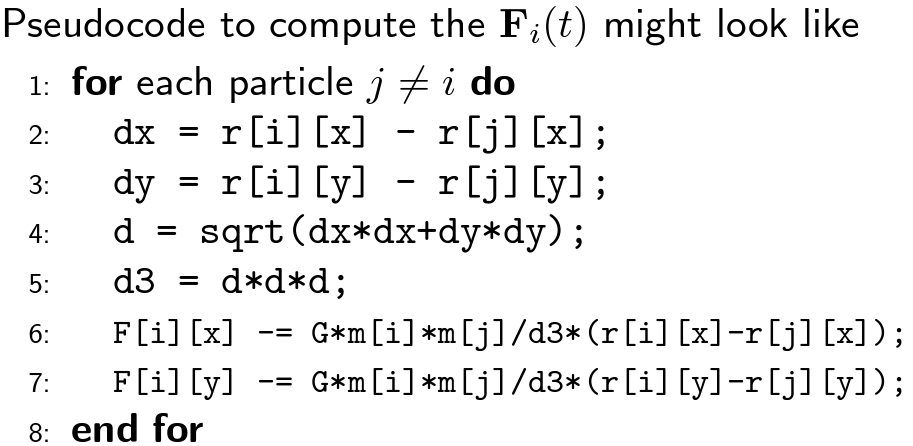
\includegraphics[width=0.75\textwidth]{pseudo-code-c}
\end{frame}

\begin{frame}
  \frametitle{Код с OpenMP}
  $f_{ij} = -f_{ji}$

  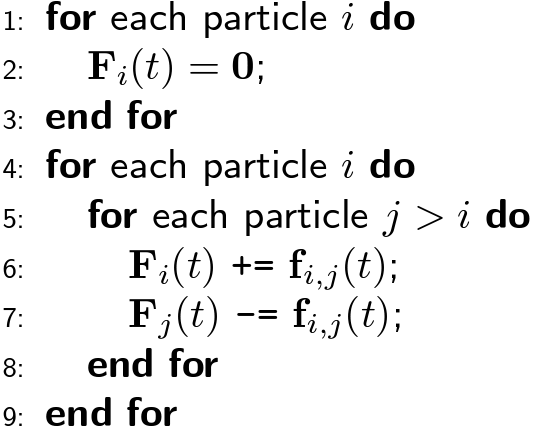
\includegraphics[width=0.45\textwidth]{pseudo-code1}
\end{frame}

\begin{frame}
  

  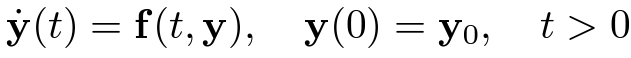
\includegraphics[width=0.65\textwidth]{ode1}  

  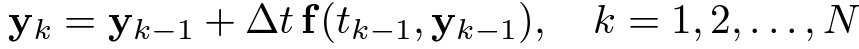
\includegraphics[width=0.89\textwidth]{ode2}  \pause

  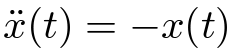
\includegraphics[width=0.24\textwidth]{ode3}

  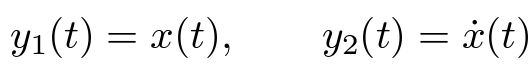
\includegraphics[width=0.5\textwidth]{ode4}
  
  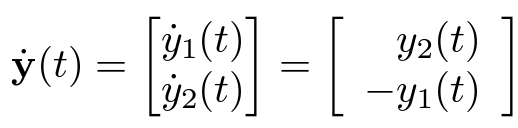
\includegraphics[width=0.5\textwidth]{ode5}
\end{frame}

\begin{frame}
  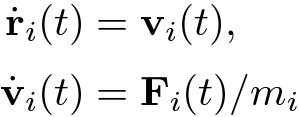
\includegraphics[width=0.3\textwidth]{ode6}

  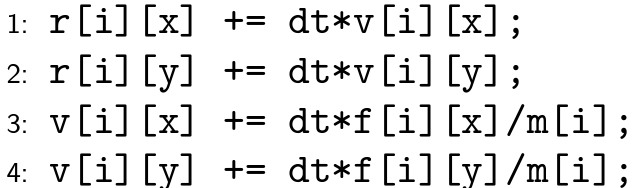
\includegraphics[width=0.5\textwidth]{pseudo-code2}
\end{frame}

\begin{frame}[fragile,plain]
  \frametitle{Сериен код за енергия}
\begin{verbatim}
for(i=0; i<nbodies; ++i)
  for(j=i+1; j<nbodies; ++j) {
    d2 = 0.0;
      for(k=0; k<3; ++k) {
        rij[k] = pos[i][k] - pos[j][k];
        d2 += rij[k]*rij[k];
      }
      if (d2 <= cut2) {
         d = sqrt(d2);
         d3 = d*d2;
         for(k=0; k<3; ++k) {
            double f = -rij[k]/d3;
      	    forces[i][k] += f;
            forces[j][k] -= f;
         }
         ene += -1.0/d; 
      }
}
\end{verbatim}

\end{frame}

\begin{frame}[fragile,plain]
  \frametitle{OpenMP код за енергия}
\scriptsize
\begin{verbatim}
#pragma omp parallel for private(i,j,k,rij,d,d2,d3) 
      reduction(+:ene) schedule(guided)
 for(i=0; i<nbodies; ++i)
  for(j=i+1; j<nbodies; ++j) {
   d2 = 0.0;
   for(k=0; k<3; ++k) {
    rij[k] = pos[i][k] - pos[j][k];
    d2 += rij[k]*rij[k];
   }
   if (d2 <= cut2) {
     d = sqrt(d2);
     d3 = d*d2;
     for(k=0; k<3; ++k) {
       double f = -rij[k]/d3;
#pragma omp atomic
       forces[i][k] += f;
#pragma omp atomic
       forces[j][k] -= f;
   }
   ene += -1.0/d;
}
\end{verbatim}
\end{frame}


\begin{frame}[fragile]{}
  Горният код е от
  \url{https://hpc-old.cineca.it/content/training-openmp}
\end{frame}

\begin{frame}
  \frametitle{Домашна работа}
  Използвайки разгледания код, както и фрагмента от слайд 9,
  определете динамиката на системата от частици с данните от
  \url{https://hpc-old.cineca.it/content/exercise-5-0}. В частност,
  определете местоположението на частиците след 5 времеви интервала.
\end{frame}

\end{document}


%%% Local Variables:
%%% mode: latex
%%% TeX-master: t
%%% End:

